\chapter{مقدمه}
\section{انقلاب صنعتی چهارم و شهر‌های هوشمند}
انقلاب صنعتی چهارم\LTRfootnote{\lr{Fourth Industry Revolution}}، جدیدترین فاز پیشرفت فناوری در صنعت و تولید است که با ادغام سیستم‌های دیجیتالی، فیزیکی و بیولوژیکی شناخته می‌شود. این انقلاب بر روی انقلاب صنعتی سوم که با بهره‌گیری از تکنولوژی کامپیوتر‌ها و اتوماسیون همراه بود، بنا شده است و با بهره‌گیری از تکنولوژی‌هایی نظیر اینترنت اشیا\LTRfootnote{\lr{Internet of Things (IoT)}}، هوش مصنوعی، رباتیک و آنالیز پیشرفته داده یک قدم به سمت جلو برداشته است.

انقلاب صنعتی چهارم به طور اساسی روش زندگی و کار ما را تغییر می‌دهد و مدل‌های جدید کسب‌و‌کار، صنایع و روش‌های تعامل آنها با یکدیگر را ایجاد می‌کند. این انقلاب به شرکت‌ها این امکان را می‌دهد که فرایند‌های خود را دیجیتالی کنند، عملیات خود را بهینه کنند و محصولات و خدمات جدیدی را ایجاد کنند که قبلاْ غیر‌قابل تصور بوده است. انقلاب صنعتی چهارم همچنین ماهیت کار کردن را تغییر می‌دهد و با پتانسیل اتوماسیون بسیاری از وظایف، کارهای روزمره و افزایش قابلیت انسان در تعامل با فناوری همراه است.

شهر‌های هوشمند یکی از هیجان‌انگیزترین و تحول‌بخش‌ترین توسعه‌های انقلاب صنعتی چهارم است. با تکیه بر تکنولوژی‌های اخیر نظیر اینترنت اشیاء، هوش مصنوعی و آنالیز داده؛ شهرهای هوشمند شیوه زندگی، کار و تعامل انسان‌ها با محیط را متحول کرده‌اند. در اصل، شهرهای هوشمند برای بهبود کیفیت زندگی شهروندان و بهبود کارایی و پایداری زیرساخت‌های شهری طراحی شده‌اند. شهرهای هوشمند در مسائلی از جمله کاهش ترافیک و آلودگی هوای شهری تا بهینه‌سازی مصرف انرژی و بهبود ایمنی عمومی نقش کلیدی دارند. شهر‌های هوشمند از داده‌های مختلف و آنالیز آن‌ها برای تصمیم‌گیری‌های بهتر و بهبود تجربه زندگی شهری بهره می‌برند.

یکی از ویژگی‌های کلیدی شهرهای هوشمند، قابلیت استفاده آن‌ها از حسگرهای پیشرفته و شبکه‌های ارتباطی برای جمع‌آوری و آنالیز داده‌ها به صورت بلادرنگ\LTRfootnote{\lr{Real-time}} است. این داده‌ها می‌توانند برای ایجاد سیستم‌های حمل‌ و نقل هوشمند که جریان ترافیک را بهینه‌ می‌کنند و ترافیک را کاهش می‌دهند، استفاده شوند.

شهرهای هوشمند یکی از بهترین‌ مثال‌های انقلاب صنعتی چهارم هستند و تاثیر آن‌ها به مرور زمان رشد می‌کند، زیرا شهر‌های بیشتری در دنیا به دیجیتالی شدن و قدرت‌ تحول‌بخش فناوری‌های پیشرفته روی می‌آورند.
\section{سیستم‌های حمل و نقل هوشمند}
سیستم‌های حمل ‌و نقل هوشمند فناوری‌ها و سیستم‌های پیشرفته‌ای هستند که برای بهینه‌سازی عملکرد، امنیت و پایداری شبکه‌های حمل و نقل طراحی شده‌اند. سیستم‌های حمل و نقل هوشمند، شامل یک مجموعه گسترده از فناوری‌ها مانند سیستم‌های مدیریت ترافیک، سیستم‌های ارتباطی خوردو به خودرو، خودرو به زیرساخت، خودرو‌های خودران و سیستم‌های کمک راننده پیشرفته است.

هدف اصلی سیستم‌های حمل و نقل هوشمند، بهبود کارایی و ایمنی شبکه‌های حمل و نقل است که کاهش تاثیرات زیست محیطی را نیز به دنبال دارد. با بهره‌گیری از داده‌های بلادرنگ و الگوریتم‌های پیشرفته، این سیستم‌ می‌تواند جریان ترافیک را بهینه کند، حمل و نقل را بهبود ببخشد و ایمنی کاربران جاده را تقویت بدهند. همچنین، این سیستم‌ها می‌توانند به کاهش تراکم ترافیک کمک کنند، که به کاهش جریان ترافیک، کاهش آلودگی و کیفیت هوای محیط کمک می‌کند.

یکی از مهم‌ترین اجزای سیستم‌های حمل و نقل هوشمند، سیستم‌های مدیریت ترافیک هستند که برای نظارت و مدیریت جریان ترافیک به صورت بلادرنگ طراحی شده‌اند. این سیستم‌ها از انواع منابع مانند حسگر‌ها، دوربین‌ها و دستگاه‌های موقعیت‌یاب\LTRfootnote{\lr{GPS}}، داده‌‌ها را جمع‌آوری می‌کنند و از آن برای تنظیم پویای زمان‌بندی سیگنال‌های ترافیکی، تغییر مسیر ترافیک و ارائه اطلاعات ترافیکی بلادرنگ به کاربران جاده استفاده می‌کنند.
در سال‌های اخیر، برای شبیه‌سازی بلادرنگ صحنه‌های ترافیکی از فناوری دوقلوی دیجیتال استفاده می‌شود تا بتوان سیستم‌های هوشمند ترافیکی را در محیطی نزدیک به واقعیت آزمود.
\section{شبیه‌سازی محیط برای سیستم‌های هوشمند مدیریت ترافیک}
شبیه‌سازی یکی از پراستفاده‌ترین روش‌ها برای تسهیل طراحی سیستم‌‌های مدیریت ترافیک است. شبیه‌ساز ماشین‌های خودران یک فضای دنیای فیزیکی را به شکل یک فضای دیجیتالی بازسازی می‌کند و این بستر آزمایشی را در اختیار سیستم‌های هوشمند مدیریت ترافیک قرار می‌دهد تا بتواند شرایط شبیه‌سازی شده را زیر نظر بگیرد، تصمیم درست در انتخاب مسیر ترافیک و سیگنال‌های ترافیکی بگیرد و عمل مناسب را انجام دهد \cite{wang2022automatic}. شبیه‌سازی، یک بستر کنترل شده و امن را برای پیاده‌سازی و آزمایش سیستم‌‌های مدیریت ترافیک فراهم می‌کند. در این روش ابتدا نرم‌افزار در فضای شبیه‌سازی شده پیاده‌سازی می‌شود و پس از آزمون‌های گوناگون و اطمینان از کارکرد آن، در دنیای فیزیکی واقعی آزموده می‌شود \cite{wang2022automatic}. اما اگر فضای شبیه‌سازی ما ایستا باشد، یعنی در شبیه‌سازی از داده‌های پویا همانند عابر پیاده، ماشین‌های دیگر، تغییرات آب و هوا و... استفاده نشود، آزمون‌های ما قابل اطمینان نخواهند بود و نمی‌توانیم سیستم طراحی شده خود برای مدیریت ترافیک را در دنیای واقعی بیازماییم. پس نیاز است از شبیه‌سازی‌های پیشرفته‌ استفاده ‌کنیم که در آن فضای شبیه‌سازی شده پویا باشد و مشابه دنیای‌ واقعی عمل کند.

\section{دوقلوی دیجیتال}
دوقلوی دیجیتال، یک بازنمایی پویا و دیجیتال از یک سیستم یا یک فضا است که توسط مایکل گریوز\LTRfootnote{\lr{Michael Grieves}} در سال 2003 معرفی شد \cite{grieves2014digital}. پس از آن این مفهوم توسط ناسا\LTRfootnote{\lr{NASA}} بازبینی شد و آن را یک شبیه‌سازی بسیار دقیق و چند لایه‌ای از یک پدیده یا یک سیستم معرفی کرد که براساس داده‌های بلادرنگ شبیه‌سازی می‌شود \cite{glaessgen2012digital}. روزن و همکاران\LTRfootnote{\lr{Rosen et al.}} در مقاله‌ای منتشر شده در سال 2015، دوقلوی دیجیتال را یک بازنمایی مجازی از دنیای فیزیکی معرفی می‌کند که با استفاده از داده‌ها و شبیه‌سازی‌ها؛ کنترل‌ و بهینه سازی را مقدور می‌سازد \cite{rosen2015importance}. از دوقلوی دیجیتال برای شبیه‌سازی، نظارت و مدیریت سیستم‌ها و پدیده‌ها استفاده می‌شود، زیرا قادر به متصل کردن دنیای فیزیکی به دنیای مجازی آنها است، به گونه‌ای که چرخه زندگی\LTRfootnote{\lr{System Lifecycle}} سیستم‌ها را به صورت کامل شبیه‌سازی می‌کند. با بکارگیری از اینترنت اشیا و قابلیت متصل کردن حسگرهای گوناگون با استفاده از اینترنت، می‌توانیم از داده‌های بلادرنگ جمع ‌آوری شده از حسگر‌ها توسط شبکه‌های ارتباطی استفاده کنیم و دوقلویی دیجیتال از سیستم‌ها و پدیده‌های گوناگون تشکیل دهیم. دوقلوی دیجیتال به تازگی در بازارهای بزرگ صنعت و شهرسازی استفاده می‌شود و شبیه‌سازی‌های بسیار دقیق آن از دنیای واقعی، پیاده‌سازی انواع سیستم‌ها و مانیتورینگ را بسیار کارآمد کرده است \cite{farsi2020digital}.

دوقلوی دیجیتال، یکی از مولفه‌های اصلی انقلاب صنعتی چهارم است، به گونه‌ای که بیشتر شرکت‌ها و کارخانه‌ها، چرخه‌های زندگی سیستم‌های خود و مدل‌های مختلفی از پدیده‌های گوناگون را دیجیتالیزه می‌کنند، یا به عبارتی دوقلویی دیجیتال می‌سازند، و تمامی طراحی‌ها و آزمایش‌های گوناگون را در این بستر انجام می‌دهند. همچنین شرکت‌های شهرسازی و دولت‌ها، در حال ساختن دوقلوی دیجیتالی از شهر‌های خود هستند تا بتوانند طرح‌های جدید را در سطح شهری بیازمایند و نتایج بدست آمده را تحلیل کنند.  

دوقلوی دیجیتال و شبیه‌سازی هر دو از مدل‌های دیجیتالی برای بازنمایی پروسه‌های مختلف یک سیستم استفاده می‌کنند. اما دوقلوی دیجیتالی یک محیط و فضای مجازی براساس واقعیت است که آن را برای تحقیقات بسیار ارزشمندتر می‌کند. یکی از تفاوت‌های دوقلوی دیجیتال و شبیه‌سازی در مقیاس آنهاست؛ با استفاده از شبیه‌سازی، عموما در مورد یک پروسه خاص تحقیق و بررسی می‌شود، اما دوقلوی دیجیتال بررسی چندین شبیه‌سازی بر روی چندین پروسه را میسر می‌کند. تفاوت دیگر شبیه‌سازی و دوقلوی دیجیتال این است که شبیه‌سازی عموما از داده‌های بلادرنگ استفاده نمی‌کند،  در حالی که دوقلوی دیجیتال از یک جریان دوطرفه اطلاعات بهره می‌برد به طوری که در ابتدا از حسگر‌ها داده‌های بلادرنگ را می‌گیرد و در دوقلوی دیجیتال شبیه‌سازی می‌کند و نتیجه حاصل را به دنیای فیزیکی و سیستم یا شئ مورد نظر بر‌می‌گرداند.

\section{دوقلوی دیجیتال در صحنه‌های شهری و ترافیکی}
دوقلو‌های دیجیتال ابزاری قدرتمند و محبوب در حیطه توسعه سیستم‌های حمل‌ و نقل هوشمند برای مدیریت صحنه‌های ترافیکی هستند. دوقلوهای دیجیتال با پیاده‌سازی بسیار دقیق و جامع از جاده‌ها و زیرساخت آن‌ها از جمله ماشین‌ها و عابرین پیاده، می‌توانند داده‌های آماری مهمی را از جاده‌ها بدست بیاورند. آنها همچنین فضایی تحت کنترل و امن را برای آزمودن مشابه واقعیت سیستم‌های طراحی شده برای کنترل جریان و تراکم ترافیک را مهیا می‌کنند. به طور مثال می‌توان به پروژه عظیم کشور چین برای ساخت دوقلوی دیجیتال شهر هوشمند بیجینگ اشاره کرد که بخش بزرگی از آن ساخت دوقلوی دیجیتال شبکه جاده‌های شهری است \cite{51World:2019}.

\begin{figure}[h]
	\centering
	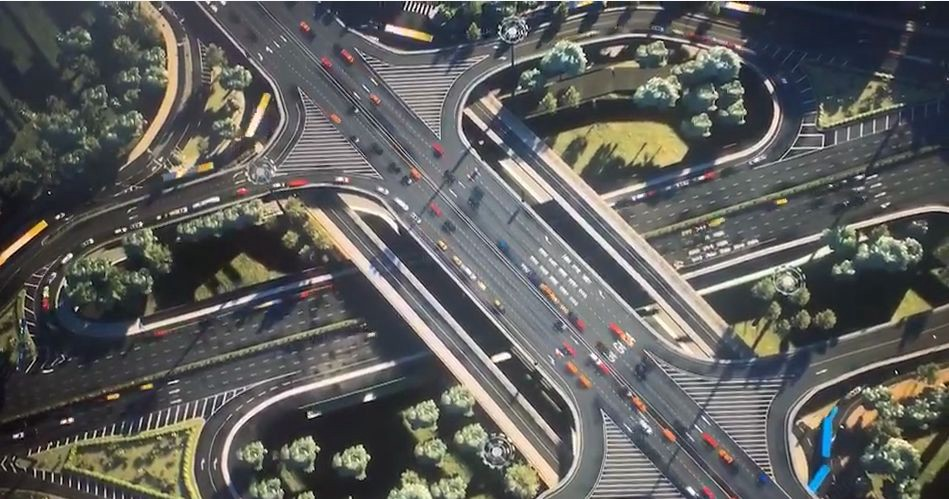
\includegraphics[scale=0.45]{figures/traffic_scene_digital_twin.jpeg}
	\caption{ تصویری از دوقلوی دیجیتال یک اتوبان در بیجینگ که به صورت زنده در حال شبیه‌سازی وضعیت کنونی اتوبان‌ است. \cite{51World:2019}}
	\label{fig:beijing_traffic_scene_dt}
\end{figure}

در \cref{fig:beijing_traffic_scene_dt}، تصویری از دوقلوی دیجیتال اتوبان بیجینگ غربی سوم\LTRfootnote{\lr{Beijing West 3rd Ring Road}} را مشاهده می‌کنیم. در این تصویر، دوقلوی دیجیتال صحنه ترافیکی علاوه بر مدل سه بعدی فضای شهری شامل خیابان‌ها و فضای سبز و دیگر المان‌های ثابت در صحنه، اطلاعات پویا مانند خودروهای در حال تردد را نیز شامل می‌شود.. حال با استفاده از این دوقلوی دیجیتال، می‌توان تراکم ترافیک در ساعات مختلف در این اتوبان دیجیتالی را به دست آورد. این اطلاعات کاربردهای متعددی می‌تواند داشته باشد. برای مثال، می‌توان از این اطلاعات بعنوان دادگانی برای آموزش مدل‌های یادگیری عمیق\LTRfootnote{\lr{Deep Learning}} استفاده کرد و تراکم ترافیک را در ساعات مختلف روز پیش‌بینی کرد. همان‌ طور که قبلاً نیز ذکر شد، دوقلوی دیجیتال می‌تواند دارای جریان دوطرفه اطلاعات باشد. به طور مثال در این اتوبان، داده‌های گرفته شده از حسگرهای مختلف همانند لایدارها\LTRfootnote{\lr{LiDAR Sensor}} و دوربین‌های مستقر (یا به عبارت دیگر یک آر.اس.یو\LTRfootnote{\lr{Road-Side Unit (RSU)}}) به عنوان ورودی دریافت می‌شوند (جریان داده دنیای واقعی به دوقلوی دیجیتال). پس از پردازش داده‌ها در دوقلوی دیجیتال و تشخیص خودروها و موقعیت مکانی آن در زمان‌های مختلف روز، مدل یادگیری عمیقی را توسعه دهیم که بتواند در راستای هوشمندسازی مدیریت ترافیک، زمان‌بندی چراغ‌های راهنمایی را بگونه‌ای کنترل کند که جریان ترافیکی بهینه شود (جریان داده‌ دوقلوی دیجیتال به دنیای واقعی).

\section{ضرورت استفاده از دوقلوی دیجیتال}
برخی از برتری‌های استفاده از دوقلوی دیجیتال به عنوان بستر شبیه‌سازی عبارتند از:

\begin{enumerate}
	\item \textbf{نزدیکی به واقعیت:} همانطور که ذکر شد، دوقلوی دیجیتال از مدل‌های پویا نیز بهره می‌برد و هدف آن نزدیکی به واقعیت تا حد امکان است. پس با مدل کردن یک صحنه ترافیکی براساس داده‌های بلادرنگ، می‌توان بستری برای سیستم‌های مدیریت ترافیک و خود‌رو‌های خودران مهیا کرد. نتایج آزمایش سیستم‌های طراحی شده در دوقلوی دیجیتال را می‌توان به دنیای واقعی نسبت داد زیرا عملا با آزمایش در دوقلوی دیجیتال، ما در بستری بسیار نزدیک به واقعیت سیستم‌ خود را آزمایش کرده‌ایم.
	\item \textbf{افزایش سرعت تحقیقات:} با بکارگیری از دوقلوی دیجیتال صحنه‌های ترافیکی، نیازی به تولید سناریو‌های مختلف ترافیکی وجود ندارد زیرا هر لحظه از دنیای واقعی در دوقلوی دیجیتال نیز در حال تشکیل است و به صورت خودکار سناریو‌های گوناگون رخ می‌دهند، در نتیجه سرعت تحقیقات و آزمایش سیستم‌های مدیریت ترافیک گوناگون به مراتب بیشتر است.
	\item \textbf{امنیت بالا:} در دوقلوی دیجیتال از مدل‌های پویا استفاده می‌شود، یعنی عابر پیاده و ماشین‌های دیگر نیز شبیه‌سازی می‌شوند و سیستم‌هایی هوشمند همچون ماشین‌های خودران و مدیریت ترافیک می‌توانند با وجود این مدل‌ها آزموده شوند. اما در دنیای واقعی آزمودن این در سطح شهر امری بسیار خطرناک است و ممکن است خسارات جبران ناپذیری بر سطح شهر وارد شود.
	\item \textbf{قابلیت پیش‌بینی بهتر:} با استفاده از دوقلوی دیجیتال، ما می‌توانیم ترافیک‌ را پیش‌بینی کنیم و نسبت به آن سیستم مدیریت ترافیک خود را تعلیم دهیم. به علت متصل بودن داده‌های دوقلوی دیجیتال به داده‌های دنیای واقعی، سناریو‌های گوناگون رخ می‌دهند و سیستم‌های مدیریت ترافیک داده‌های تمرینی بهتر و متنوع‌تر خواهند داشت \cite{singh2021digital}.
\end{enumerate}

\section{تعریف مسئله}
مشاهده کردیم که کشور چین، دوقلوی دیجیتال یکی از اتوبان‌های خود را در سال ۲۰۲۱ با موفقیت پیاده‌سازی کرد و در حال تحقیق بر روی این موضوع است. با الهام گرفتن از این پروژه، اهداف این پژوهش را در دو دسته‌ی هدف اصلی و اهداف فرعی بخش‌بندی می‌کنیم.

\subsection{هدف اصلی}

هدف اصلی این پروژه، پیاده‌سازی دوقلوی دیجیتالی از صحنه ترافیکی خیابان رشت، از دید درب رشت دانشگاه صنعتی امیرکبیر است. این دوقلوی دیجیتال به عنوان یک بازنمایی دقیق و پویا از خیابان رشت ایجاد می‌شود تا امکان شبیه‌سازی و مطالعه وضعیت‌های ترافیکی مختلف در این منطقه را فراهم کند. (مشابه دوقلوی دیجیتال اتوبان بیجینگ با جزییات به مراتب ساده‌تر)

\subsection{اهداف فرعی}

برای دستیابی به هدف اصلی پروژه، اهداف فرعی زیر تعیین شده‌اند:

\begin{enumerate}
\item مدل‌سازی ایستای سه‌بعدی خیابان رشت با استفاده از نرم‌افزارهای طراحی سه‌بعدی مبتنی بر برداشت داد‌ه‌های حسگر لایدار (به صورت دستی با کمک نرم‌افزارهای طراحی سه‌بعدی)
\item مستقر کردن حسگر‌های لایدار و دوربین در محل نگهبانی درب رشت دانشگاه صنعتی امیرکبیر به منظور برداشت داده‌های پویا.
\item پردازش داده‌های تصویر و ابر نقاط\LTRfootnote{\lr{Point Cloud (PCL)}} به منظور شناسایی و مکانیابی پدیده‌های پویا با استفاده از مدل‌های آماده یادگیری ماشین در زمینه تشخیص اجسام سه‌بعدی.
\item بصری‌سازی مدل سه‌بعدی ایستا و داده‌های پویای شناسایی شده در بستر سه‌بعدی با استفاده از شبیه‌ساز \lr{AWSIM}.
\item بصری‌سازی اطلاعات آماری بدست آمده از دوقلوی دیجیتال به منظور تجزیه و تحلیل نتایج پروژه.
\end{enumerate}

این اهداف فرعی به منظور دستیابی به هدف اصلی پروژه ارائه شده‌اند و با استفاده از آنها، پروژه به طور جامع توصیف و اجرا می‌شود.